%%%%%%%%%%%%%%%%%%%%%%%%%%%%%%%%%%%%%%%%%%%%%%%%%%%%%%%%%%%%%%%%%%%%%%%%%%%%%%%%
% AMS Beamer series / Bologna FC / Template
% Andrea Omicini
% Alma Mater Studiorum - Università di Bologna
% mailto:andrea.omicini@unibo.it
%%%%%%%%%%%%%%%%%%%%%%%%%%%%%%%%%%%%%%%%%%%%%%%%%%%%%%%%%%%%%%%%%%%%%%%%%%%%%%%%
%\documentclass[handout]{beamer}\mode<handout>{\usetheme{default}}
%
\documentclass[presentation]{beamer}\mode<presentation>{\usetheme{AMSBolognaFC}}
%\documentclass[handout]{beamer}\mode<handout>{\usetheme{AMSBolognaFC}}
%%%%%%%%%%%%%%%%%%%%%%%%%%%%%%%%%%%%%%%%%%%%%%%%%%%%%%%%%%%%%%%%%%%%%%%%%%%%%%%%
\usepackage{ske-ski-talk-2022}
%%%%%%%%%%%%%%%%%%%%%%%%%%%%%%%%%%%%%%%%%%%%%%%%%%%%%%%%%%%%%%%%%%%%%%%%%%%%%%%%
\title[Dive into \skeski]
{Dive into \longskeski}
%
\subtitle[gentle introduction and technologies]
{gentle introduction and technologies}
%

\author[\sspeaker{Magnini et al.} ]
{\speaker{Matteo Magnini}$^{*}$ \and Giovanni Ciatto$^{*}$}
%
\institute[DISI, Univ.\ Bologna]
{
    $^{*}$Dipartimento di Informatica -- Scienza e Ingegneria (DISI)\\\textsc{Alma Mater Studiorum} -- Universit{\`a} di Bologna
    \\
    \{\speaker{matteo.magnini}, giovanni.ciatto\}@unibo.it % emph the presenting author's email
}
%
\date[XAI project]{XAI project\\October 7, 2022, virtual}
%
\AtBeginSection[]
{
    %\\\\\\\\\\\\\\\\\\\\\
    \begin{frame}<beamer>[c,noframenumbering]
        \frametitle{Next in Line\ldots}
        \tableofcontents[sectionstyle=show/shaded,subsectionstyle=hide]
    \end{frame}
    %\\\\\\\\\\\\\\\\\\\\\
}
\AtBeginSubsection[]
{
    %\\\\\\\\\\\\\\\\\\\\\
    \begin{frame}<beamer>[shrink,noframenumbering]
        \frametitle{Focus on\ldots}
        \mbox{~}
        \tableofcontents[currentsubsection,sectionstyle=shaded,subsectionstyle=show/shaded]
        \mbox{~}
    \end{frame}
    %\\\\\\\\\\\\\\\\\\\\\
}
%
%%%%%%%%%%%%%%%%%%%%%%%%%%%%%%%%%%%%%%%%%%%%%%%%%%%%%%%%%%%%%%%%%%%%%%%%%%%%%%%%
\begin{document}
%%%%%%%%%%%%%%%%%%%%%%%%%%%%%%%%%%%%%%%%%%%%%%%%%%%%%%%%%%%%%%%%%%%%%%%%%%%%%%%%

%/////////
\frame{\titlepage}
%/////////

%%===============================================================================
%\section*{Outline}
%%===============================================================================
%
%%/////////
%\frame[c]{\tableofcontents[hideallsubsections]}
%%/////////


%===============================================================================
\section{Premises}
%===============================================================================

\begin{frame}[c]{Presentation}
    
    \begin{block}{Not only myself}
        \begin{itemize}
            \item \emph{Andrea Agiollo}, \unibo{} \disi{};
            %
            \item \emph{Andrea Omicini}, \unibo{} \disi{};
            %
            \item \emph{Andrea Rafanelli}, \unipi{} \di{}, \uniaq{} \disim{};
            %
            \item \emph{Federico Sabbatini}, \uniurb{} \dispea{};
            %
            \item \emph{Giovanni Ciatto}, \unibo{} \disi{};
            %
            \item \emph{Matteo Magnini}, \unibo{} \disi{};
        \end{itemize}
    \end{block}

\end{frame}

\begin{frame}[allowframebreaks]{Concerning human (and machine) reasoning}
    
    \begin{block}{The three ways}
        \begin{itemize}
            \item \alert{induction} $\rightarrow$ a kind of reasoning that uses particular examples in order to reach a general conclusion about something;
            %
            \item \alert{deduction} $\rightarrow$ the act or process of using logic or reason to form a conclusion or opinion about something;
            %
            \item \alert{abduction} $\rightarrow$ the forming and accepting on probation of a hypothesis to explain surprising facts.
        \end{itemize}
    \end{block}

    \framebreak
    
     \begin{block}{The three ways}
        \begin{itemize}
            \item \alert{induction} $\rightarrow$ machine learning (e.g., neural networks);
            %
            \item \alert{deduction} $\rightarrow$ symbolic artificial intelligence (e.g., logic programs);
            %
            \item \alert{abduction} $\rightarrow$ abductive logic programming.
        \end{itemize}
    \end{block}

\end{frame}


\begin{frame}[allowframebreaks]{Concepts we need to know}

    %
    \begin{block}{Symbolic knowledge}
        A symbolic representation of knowledge consists of: \ccite{sub-symbolic-vs-symbolic}
        %
        \begin{enumerate}
            \item a set of symbols;
            \item\label{item:symbolic-combination} a set of grammatical rules governing the combining of symbols; 
            \item\label{item:symbolic-assignment} elementary symbols and any admissible combination of them can be assigned with meaning.
            %
            \begin{itemize}
                \item[$\Rightarrow$] Symbolic knowledge is both human and machine interpretable,
                \item first order logic (FOL) is an example of symbolic representation.
            \end{itemize}
        \end{enumerate}
    \end{block}
    
    \framebreak

    %/////////
    \begin{block}{Sub-symbolic data}
    \begin{itemize}
        \item ML methods, and sub-symbolic approaches in general, represent data as arrays of real numbers, and knowledge as functions over such data;
        %
        \item despite numbers are technically symbols as well, we cannot consider arrays and their functions as symbolic knowledge representation (KR) means;
        %
        \item sub-symbolic approaches frequently violate \Cref{item:symbolic-combination,item:symbolic-assignment}.
        %
    \end{itemize}
    %
    \end{block}
    %/////////
    
    \framebreak
    
    %
    \begin{block}{Local representation}
        \begin{itemize}
            \item Each number of the array has a well-defined meaning;
            %
            \item example $\rightarrow$ iris dataset sample, array with 5 elements where each element has meaning (sepal/petal length/width and class).
        \end{itemize}    
    \end{block}

    \begin{block}{Distributed representation}
        \begin{itemize}
            \item Each number of the array is meaningless, unless it is considered along with its neighbourhood;
            %
            \item example $\rightarrow$ images represented as $w\ x\ h$ matrices of numbers in range $[0,1]$.
            %
            (Violation of \cref{item:symbolic-assignment})
        \end{itemize}
    \end{block}
    
    \framebreak
    
     \begin{figure}
        \centering
        \subfloat{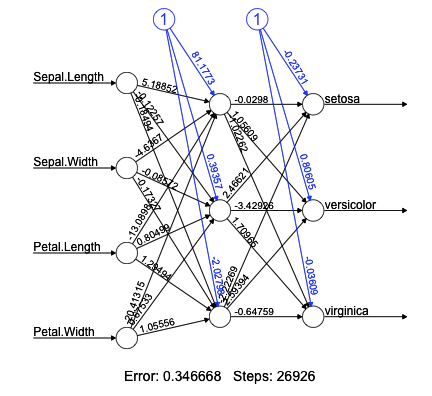
\includegraphics[width=0.4\textwidth]{figures/nn-iris}}
        %
        \qquad
        %
        \centering
        \subfloat{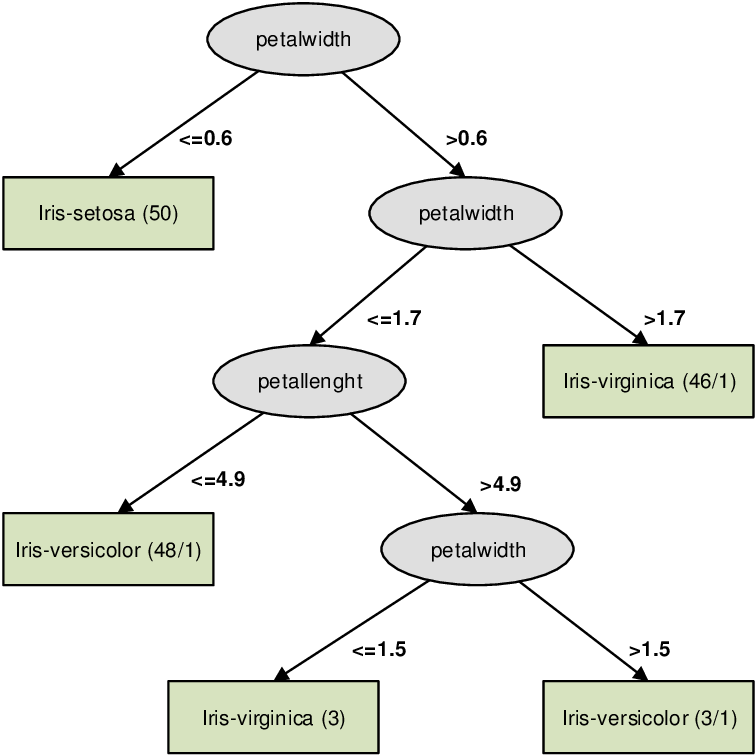
\includegraphics[width=0.4\textwidth]{figures/decision-tree-iris}}
    \end{figure}
    
    \framebreak
    
    Set of propositional logic rules built from the previous decision tree:
    
    \begin{equation*}
        \begin{aligned}
            \pred{iris}&(\var{SepalLenght}, \var{SepalWidth}, \var{PetalLenght}, \var{PetalWidth}, \const{setosa})\text{:-}\\
            &\var{PetalWidth} =< 0.6.\\
            \pred{iris}&(\var{SepalLenght}, \var{SepalWidth}, \var{PetalLenght}, \var{PetalWidth}, \const{versicolor}) \text{:-}\\
            &\var{PetalWidth} > 0.6, \var{PetalWidth} =< 1.7, \var{PetalLenght} =< 4.9.\\
            \pred{iris}&(\var{SepalLenght}, \var{SepalWidth}, \var{PetalLenght}, \var{PetalWidth}, \const{virginica}) \text{:-}\\
            &\var{PetalWidth} > 0.6, \var{PetalWidth} =< 1.5, \var{PetalLenght} > 4.9.\\
            \pred{iris}&(\var{SepalLenght}, \var{SepalWidth}, \var{PetalLenght}, \var{PetalWidth}, \const{versicolor}) \text{:-}\\
            &\var{PetalWidth} > 1.5, \var{PetalWidth} =< 1.7, \var{PetalLenght} > 4.9.\\
            \pred{iris}&(\var{SepalLenght}, \var{SepalWidth}, \var{PetalLenght}, \var{PetalWidth}, \const{virginica}) \text{:-}\\
            &\var{PetalWidth} > 1.7.\\
        \end{aligned}
    \end{equation*}
    
    \framebreak
    
\end{frame}
%/////////


%===============================================================================
\section{\longske}
%===============================================================================


%/////////
\begin{frame}[c]{Definition}
    \begin{block}{We define \longske{} (\ske) as:}
        \begin{displayquote}\itshape
            any \emph{algorithmic} procedure accepting \emph{trained} \alert{sub-symbolic predictors} as input and producing \alert{symbolic knowledge} as output, in such a way that the extracted knowledge \emph{reflects} the behaviour of the predictor with high fidelity.
        \end{displayquote}
        %
    \end{block}
    %
    \begin{block}{Notes}
        \begin{itemize}
            \item This will be just a brief introduction, I will focus more on \longski{} rather than \longske;
            %
            \item for more details and questions about \ske{} please contact \emph{Federico Sabbatini} \href{mailto:f.sabbatini@unibo.it}{f.sabbatini@unibo.it}
        \end{itemize}
    \end{block}
    
\end{frame}
%/////////







%===============================================================================
\section{\longski}
%===============================================================================
    
%/////////
\begin{frame}[c]{Definition}
    \begin{block}{We define \longski{} as: \ccite{surveyNeuroSymb,surveyXie,surveyCalegariCO20}}
        \begin{displayquote}\itshape
            any \emph{algorithmic} procedure affecting how \alert{sub-symbolic predictors} draw their inferences in such a way that predictions are either \emph{computed} as a function of, or made \emph{consistent} with, some \emph{given} \alert{symbolic knowledge}.
        \end{displayquote}
    \end{block}
    
\end{frame}
%/////////


%/////////
\begin{frame}[allowframebreaks]{Why SKI?}
    \begin{block}{There are several benefits:}
        %
        \begin{itemize}
            %
            \item prevent the predictor to become a black-box\alert{!};
            %
            \item reduce learning time;
            %
            \item reduce the data size needed for training;
            %
            \item improve predictor's accuracy;
            %
            \item build a predictor that behave as a logic engine.
        \end{itemize}
        %
    \end{block}

     \framebreak

    Explainability \ccite{darpa2016-xai} can be achieved:
    %
    \begin{block}{Post-hoc explanation}
        \begin{itemize}
            \item applying an algorithm of symbolic knowledge extraction on a trained predictor;
            %
            \item output $\rightarrow$ logic rules that describe the predictor's behaviour.
            %
        \end{itemize}    
    \end{block}
    
    \begin{block}{By design}
        \begin{itemize}
            \item constraining the behaviour of predictors that are natively black-boxes with symbolic knowledge;
            %
            \item structuring the predictor's architecture with symbolic knowledge;
            %
            \item output $\rightarrow$ a predictor that does not violate the prior knowledge.
        \end{itemize}
    \end{block}
    
\end{frame}
%/////////

\begin{frame}[c]{Taxonomy}
    \begin{block}{Dimensions}
        \begin{itemize}
            \item Aim $\rightarrow$ main purpose of the injection;
            \item Predictors $\rightarrow$ target of the injection;
            \item How $\rightarrow$ in which way the injection is performed;
            \item Logic $\rightarrow$ what kind of logic formalism is used to represent knowledge.
        \end{itemize}
    \end{block}
\end{frame}
    
\begin{frame}[c]{Aim}
    \begin{block}{Enrich (learning support)}
        \begin{itemize}
            \item reduce learning time;
            %
            \item reduce the data size needed for training;
            %
            \item improve predictor's accuracy.
        \end{itemize}
    \end{block}
    %
    \begin{block}{Manifold (symbolic knowledge manipulation)}
    \begin{itemize}
        \item logic inference;
        %
        \item information retrieval;
        %
        \item knowledge base completion/fusion.
    \end{itemize}
    \end{block}
\end{frame}
%/////////

\begin{frame}[c]{Predictors}
    \begin{block}{What kind of predictors are feasable for \ski?}
        \begin{itemize}
            \item in theory every sub-symbolic predictors;
            %
            \item in particular (deep) neural networks are the preferred targets for several reasons:
            %
            \begin{itemize}
                \item easy to manipulate;
                %
                \item high performance;
                %
                \item technological maturity.
            \end{itemize}
        \end{itemize}
    \end{block}
\end{frame}
%/////////


%/////////
\begin{frame}[allowframebreaks]{How}
    \begin{block}{Injection families}
        %
        There exist three major ways to perform knowledge injection on sub-symbolic predictors:
        %
        \begin{itemize}
            \item \alert{constraining}, a cost factor proportional to the violation of the knowledge is introduced during learning;
            \item \alert{structuring}, the architecture of the predictor is built in such a way to mimic the knowledge;
            \item \alert{embedding}, the symbolic knowledge is embedded into a tensor form and it is given in input as training data to the predictor.
        \end{itemize} 
    \end{block}
    %
    
    \framebreak

    \begin{block}{Constraining}
       \begin{itemize}
           \item Knowledge cost factor is introduced in the loss function;
           %
           \item for NN the cost affects backpropagation \ccite{backpropagation} during training.
           %
           \begin{itemize}
               \item[$\Rightarrow$] Predictor does not violate the prior knowledge (to a certain extent).
           \end{itemize} 
       \end{itemize}
       
       \begin{figure}
           \centering
           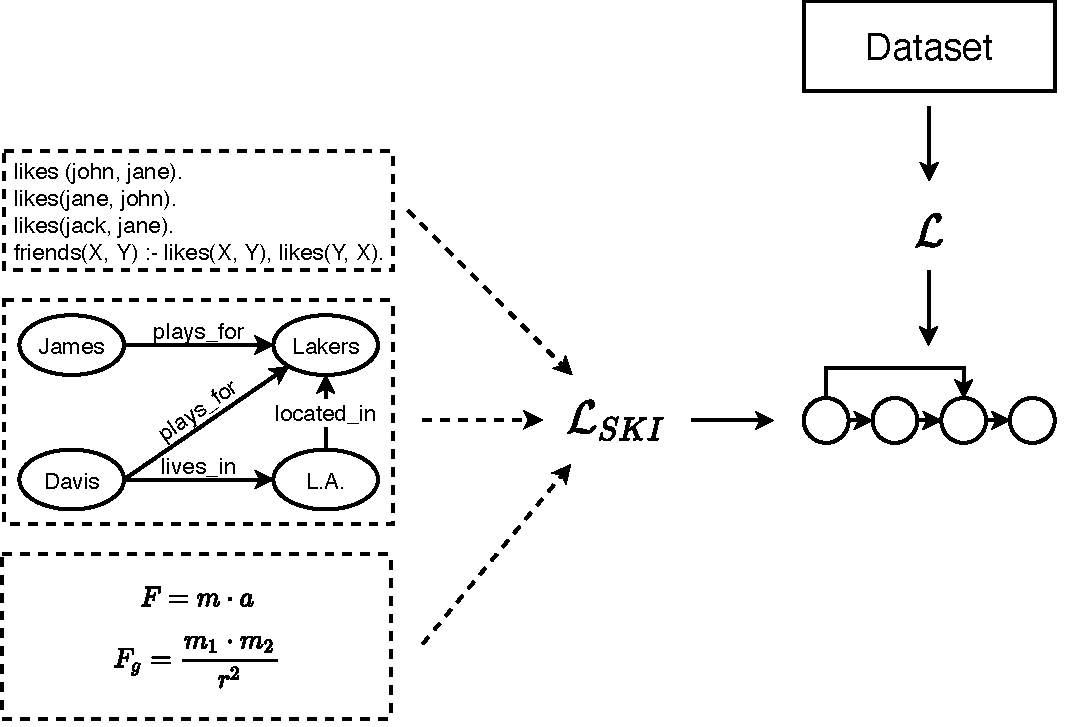
\includegraphics[width=0.4\textwidth]{figures/ski-constraining}
       \end{figure}
       %
    \end{block}
    
    \framebreak
    
    \begin{block}{Structuring}
         \begin{itemize}
            \item Inner architecture is shaped to be able to ``mimic'' the knowledge;
            %
            \item for NN this means \emph{ad-hoc} layers.
            %
            \begin{itemize}
                \item[$\Rightarrow$] Predictor directly exploits knowledge when needed.
            \end{itemize} 
        \end{itemize}
        %
        \begin{figure}
            \centering
            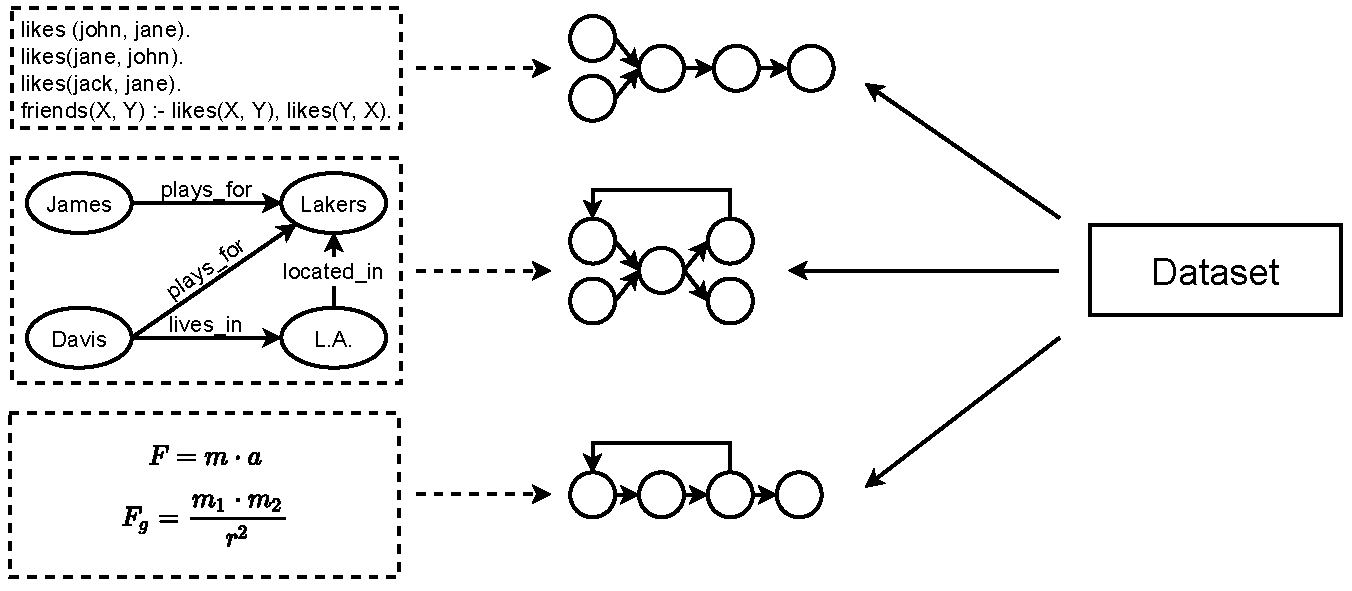
\includegraphics[width=0.6\textwidth]{figures/ski-structuring}
        \end{figure}
        %
    \end{block}

    \framebreak
   
    %
    \begin{block}{Embedding}
        \begin{itemize}
            \item Symbolic knowledge is embedded into a tensor form;
            %
            \item this is used as predictor's input data (alone or with a ``standard'' dataset).
            %
            \begin{itemize}
                \item[$\Rightarrow$] Predictor's aim is manifold in most cases.
            \end{itemize} 
        \end{itemize}
        
        \begin{figure}
            \centering
            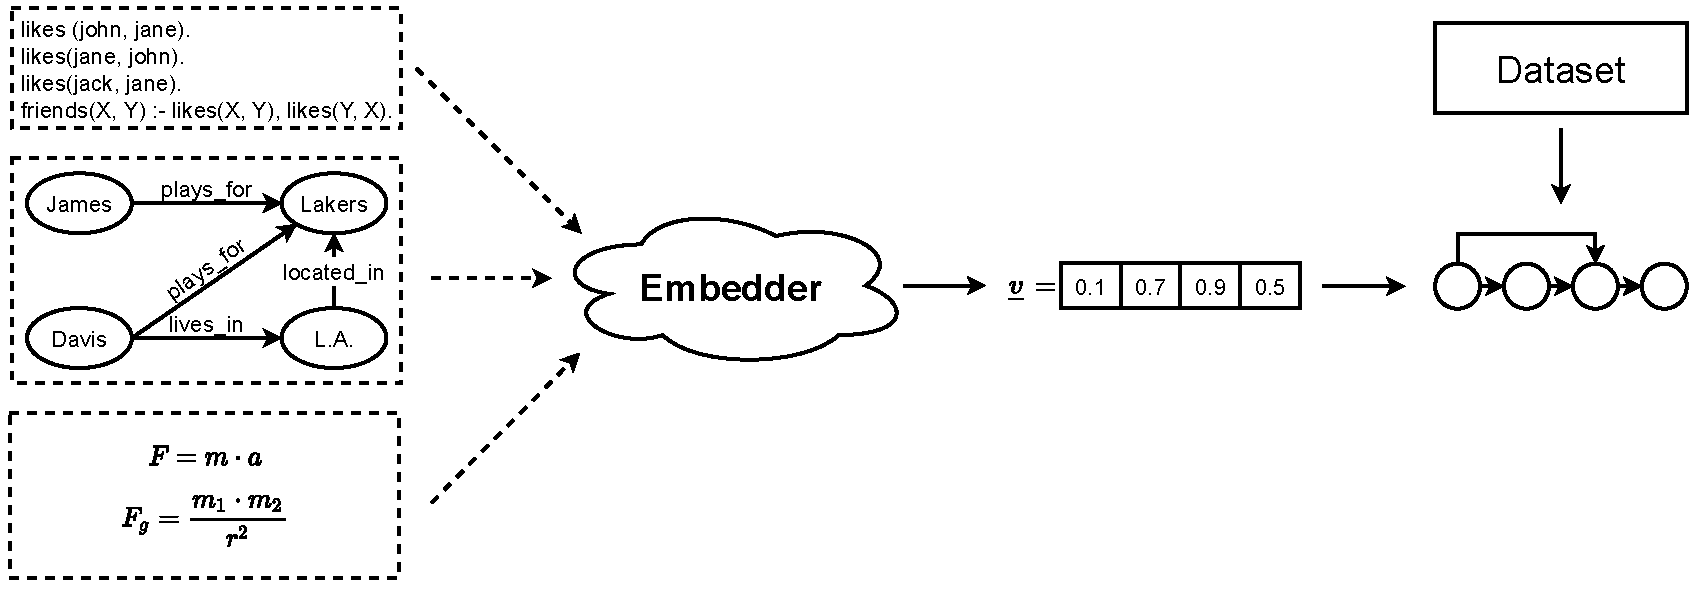
\includegraphics[width=0.6\textwidth]{figures/ski-embedding}
        \end{figure}
    \end{block}
\end{frame}
%/////////


\begin{frame}[allowframebreaks]{Logic}
    \begin{block}{Intensional}
        \begin{itemize}
            \item indirect representation of data,
            %
            \item define a relation/set by describing its elements via other relations/sets.
        \end{itemize}
        %
    \end{block}
    %
    \begin{block}{Extensional}
        \begin{itemize}
            \item direct representation of data,
            %
            \item explicit definition of entities involved.
        \end{itemize}
    \end{block}
    
    \framebreak
    
    \begin{block}{Most used logic formalisms}
        \begin{itemize}
            \item Recursive intensional predicates are very expressive and powerful, as they enable the description of infinite sets via a finite (and commonly small) amount of formul\ae;
            \item however, most sub-symbolic predictors are NN, the vast majority of them are direct acyclic graph (DAG) $\rightarrow$ no support to recursion;
            \item therefore one of the most common logic is just \alert{propositional logic (PL)} followed by \alert{knowledge graph (KG)} and then by \alert{first order logic (FOL)}.
        \end{itemize}
    \end{block}
\end{frame}



%===============================================================================
\section{\longpsyki}
%===============================================================================


\begin{frame}[c]{Gentle presentation}
    \begin{block}{\longpsyki{} (\psyki)}
        \begin{itemize}
            \item \psyki is intended as a library of \ski{} algorithms for data/computer scientists;
            %
            \item it is written in Python and supports Tensorflow;
            %
            \item code is public available on \href{https://github.com/psykei/psyki-python}{https://github.com/psykei/psyki-python}
            %
            \item to install run \texttt{pip install psyki}
            %
            \item currently \psyki{} supports the following \ski{} algorithms:
            \begin{itemize}
                \item \longkins{} (\kins);
                \item \longkill{} (\shortkill);
                \item \longkbann{} (\kbann).
            \end{itemize}
        \end{itemize}
    \end{block}
\end{frame}



%/////////
\begin{frame}[allowframebreaks]{Knowledge Injection via Network Structuring}
    
    \begin{block}{KINS: Knowledge Injection via Network Structuring}
        %
        A general SKI algorithm that does not impose constrains on the sub-symbolic predictor to enrich.
        %
        \begin{itemize}
            %
            \item aim $\rightarrow$ enrich;
            %
            \item predictor $\rightarrow$ neural network;
            %
            \item how $\rightarrow$ structuring;
            %
            \item logic $\rightarrow$ stratified Datalog with negation.
            %    
        \end{itemize}        
    \end{block}
    
    \framebreak
    
    \begin{figure}
        \centering
        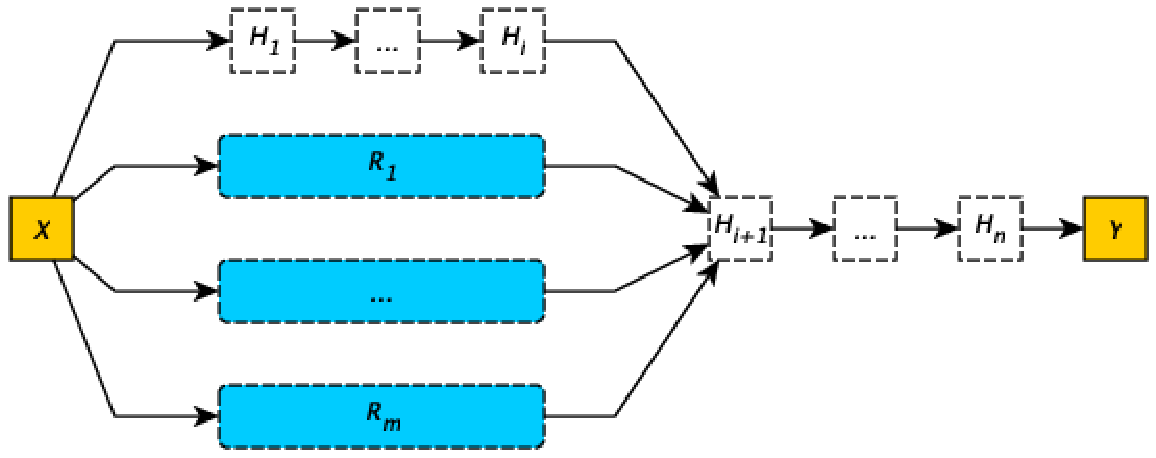
\includegraphics[width=0.8\textwidth]{figures/kins-architecture}
    \end{figure}
    
    \framebreak
    
    \resizebox{\textwidth}{!}{
    \begin{tabular}{l|r||l|r}
        \textbf{Formula} & \textbf{C. interpretation} & \textbf{Formula} & \textbf{C. interpretation}
        \\
        \hline\hline
        $\llbracket\neg \phi\rrbracket$ & $\eta\{1 - \llbracket\phi\rrbracket\}$ & $\llbracket\phi \leftarrow \psi\rrbracket$ & $\eta\{min\{1, 1-\llbracket\phi\rrbracket+\llbracket\psi\rrbracket\}\}$ % Negation % Left Implication
        \\
        $\llbracket\phi  \wedge \psi\rrbracket$ &  $\eta\{min\{\llbracket\phi\rrbracket, \llbracket\psi\rrbracket\}\}$ & $\llbracket\phi \leftrightarrow \psi\rrbracket$ & $\eta\{min\{1, 1-|\llbracket\phi\rrbracket-\llbracket\psi\rrbracket|\}\}$ % Conjunction % Double Implication
        \\
        $\llbracket\phi  \vee \psi\rrbracket$ & $\eta\{max\{\llbracket\phi\rrbracket, \llbracket\psi\rrbracket\}\}$ & $\llbracket \text{expr}(\bar{X}) \rrbracket$ & $\text{expr}(\llbracket\bar{X}\rrbracket)$ % Disjunction
        \\
        $\llbracket\phi = \psi\rrbracket$ & $\eta\{\llbracket\neg( \phi \ne \psi )\rrbracket \}$ &$\llbracket \mathtt{true} \rrbracket$ & $1$ % Equal
        \\
        $\llbracket\phi \ne \psi\rrbracket$ & $\eta\{|\llbracket\phi\rrbracket-\llbracket\psi\rrbracket|\}$ & $\llbracket \mathtt{false} \rrbracket$ & $0$ % Not Equal
        \\
        $\llbracket\phi > \psi\rrbracket$ & $\eta\{max\{0, \llbracket\phi\rrbracket - \llbracket\psi\rrbracket\}\}$ & $\llbracket X \rrbracket$ & $x$ % Greater
        \\
        $\llbracket\phi \ge \psi\rrbracket$  & $\eta\{\llbracket( \phi > \psi ) \vee ( \phi = \psi )\rrbracket\}$ & $\llbracket \const{k} \rrbracket$ & $k$ % Greater Equal
        \\
        $\llbracket\phi < \psi\rrbracket$  &  $\eta\{max\{0, \llbracket\psi\rrbracket - \llbracket\phi\rrbracket\}\}$ & $\llbracket \pred{p}(\bar{X}) \rrbracket^{**}$ & $\llbracket \psi_1 \vee \ldots \vee \psi_k \rrbracket$ % Less
        \\
        $\llbracket\phi \le \psi\rrbracket$  & $\eta\{\llbracket( \phi < \psi ) \vee ( \phi = \psi )\rrbracket\}$ & $\llbracket \pred{class}(\bar{X}, \const{y}_i) \leftarrow \psi \rrbracket$ & $\llbracket \psi \rrbracket^{*}$ % Less Equal
        \\
        $\llbracket\phi \rightarrow \psi\rrbracket$ & $\eta\{min\{1, 1- \llbracket\psi\rrbracket+\llbracket\phi\rrbracket\}\}$ & & % Right Implication        
    \end{tabular}
}
\begin{center}\scriptsize
    $^{*}$ encodes the value for the $i^{th}$ output
    \\
    \smallskip
    $^{**}$ assuming $p$ is defined by $k$ clauses of the form:
    \\
    $\pred{p}(\bar{X}) \leftarrow \psi_1,\ \ldots,\ \pred{p}(\bar{X}) \leftarrow \psi_k$
\end{center}
    
    \framebreak
    
    \begin{figure}
        \centering
        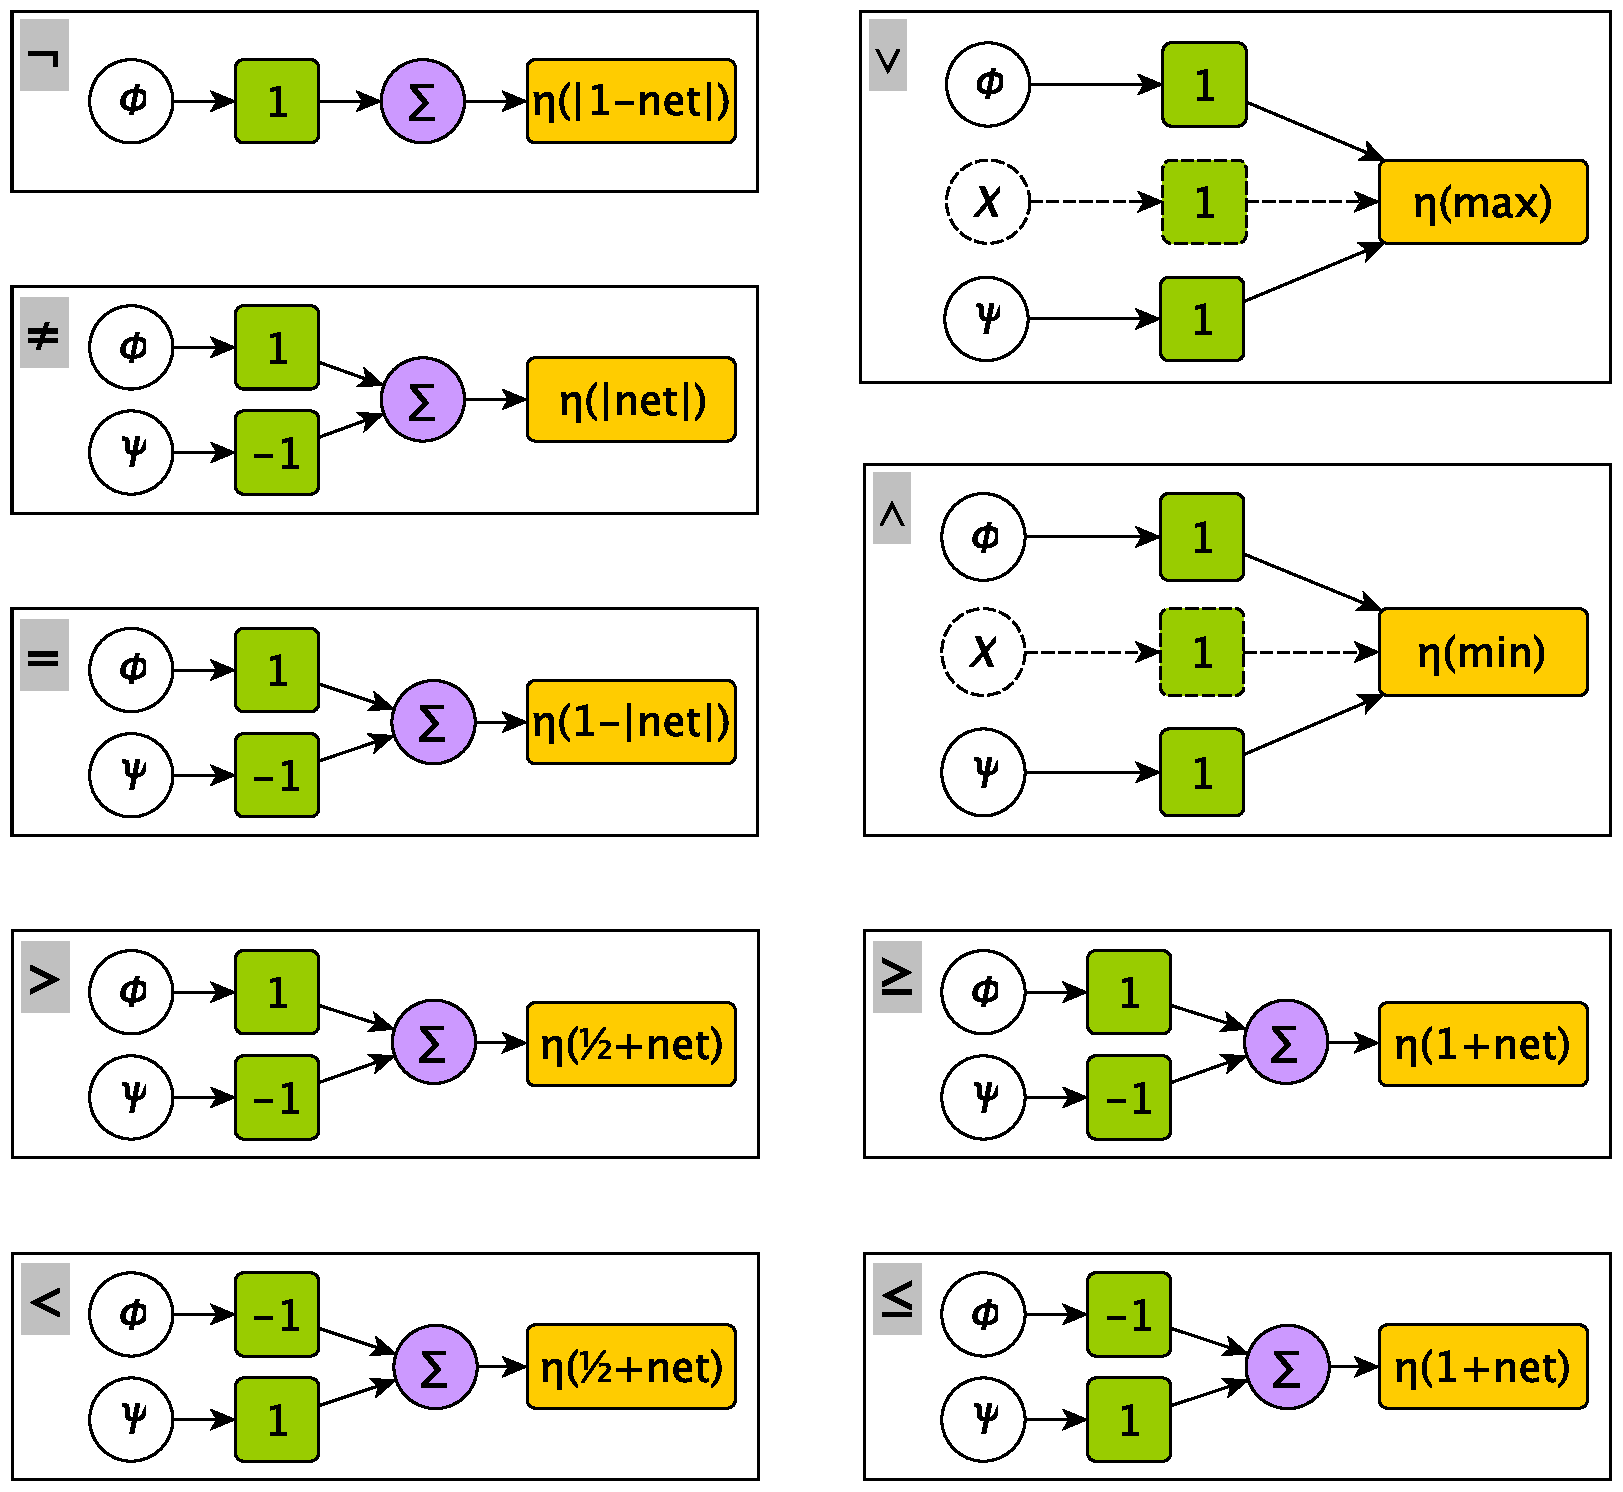
\includegraphics[width=0.65\textwidth]{figures/neurons}
    \end{figure}
    
\end{frame}
%/////////

%/////////
\begin{frame}[fragile,allowframebreaks]{Case study}
    %
    PSJGS: Primate Splice-Junction Gene Sequences dataset
    %
    \begin{minipage}{0.5\textwidth}
        \begin{lstlisting}[language={}, basicstyle=\ttfamily\tiny,frame=none]
        EI-stop ::- @-3 'TAA'.
        EI-stop ::- @-3 'TAG'.
        EI-stop ::- @-3 'TGA'.
        EI-stop ::- @-4 'TAA'.
        EI-stop ::- @-4 'TAG'.
        EI-stop ::- @-4 'TGA'.
        EI-stop ::- @-5 'TAA'.
        EI-stop ::- @-5 'TAG'.
        EI-stop ::- @-5 'TGA'.
        
        IE-stop ::- @1 'TAA'.
        IE-stop ::- @1 'TAG'.
        IE-stop ::- @1 'TGA'.
        IE-stop ::- @2 'TAA'.
        IE-stop ::- @2 'TAG'.
        IE-stop ::- @2 'TGA'.
        IE-stop ::- @3 'TAA'.
        IE-stop ::- @3 'TAG'.
        IE-stop ::- @3 'TGA'.
        
        pyramidine-rich :- 6 of (@-15 'YYYYYYYYYY').
        
        EI :- @-3 'MAGGTRAGT', not(EI-stop).
        
        IE :- pyramidine-rich, @-3 'YAGG', not(IE-stop).
        \end{lstlisting}
    \end{minipage}
    \vline
    \begin{minipage}{0.45\textwidth}
        \begin{lstlisting}[language={}, basicstyle=\ttfamily\tiny,frame=none]           
    Class, Id, DNA-sequence
    
    EI,ATRINS-DONOR-521,CCAGCTGCAT...AGCCAGTCTG
    EI,ATRINS-DONOR-905,AGACCCGCCG...GTGCCCCCGC
    EI,BABAPOE-DONOR-30,GAGGTGAAGG...CACGGGGATG
    ...
    IE,ATRINS-ACCEPTOR-701,TTCAGCGGCC...GCCCTGTGGA
    IE,ATRINS-ACCEPTOR-1678,GGACCTGCTC...GGGGGCTCTA
    IE,BABAPOE-ACCEPTOR-801,GCGGTTGATT...AAGATGAAGG
    ...
    N,AGMKPNRSB-NEG-1,CAAAAGAACA...CAAGGCTACA
    N,AGMORS12A-NEG-181,AGGGAGGTGT...GGGCATGGGG
    N,AGMORS9A-NEG-481,TGGTCAATTC...TCTTGCTCTG
    ...
    
    3190 Records
        \end{lstlisting}
    \end{minipage}
    
    \framebreak
    
    \centering
\resizebox*{!}{0.8\textheight}{
    \centering
    \begin{adjustbox}{width=\linewidth, center}
        \centering
        \begin{tabular}{c|l}
            \centering
            \textbf{Class} & \textbf{Logic Formulation}
            \\\hline\hline
            \emph{EI} & $\begin{array}{l}
                \begin{aligned}
                    \pred{class}(\bar{\var{X}}, \const{ei}) \leftarrow& \var{X}_{-3} = \const{m} \wedge \var{X}_{-2} = \const{a} \wedge \var{X}_{-1} = \const{g} \wedge \var{X}_{+1} = \const{g}\ \wedge\\
                    & \var{X}_{+2} = \const{t} \wedge \var{X}_{+3} = \const{a} = \const{r} \wedge \var{X}_{+4} = \const{a}\ \wedge \\
                    & \var{X}_{+5} = \const{g} \wedge \var{X}_{+6} = \const{t} \wedge \neg(\pred{ei\_stop}(\bar{\var{X}}))
                \end{aligned}
                \\
                \pred{ei\_stop}(\bar{\var{X}}) \leftarrow \var{X}_{-3} = \const{t} \wedge \var{X}_{-2} = \const{a} \wedge \var{X}_{-1} = \const{a}
                \\
                \pred{ei\_stop}(\bar{\var{X}}) \leftarrow \var{X}_{-3} = \const{t} \wedge \var{X}_{-2} = \const{a} \wedge \var{X}_{-1} = \const{g}
                \\
                \pred{ei\_stop}(\bar{\var{X}}) \leftarrow \var{X}_{-3} = \const{t} \wedge \var{X}_{-2} = \const{g} \wedge \var{X}_{-1} = \const{a}
                \\
                \pred{ei\_stop}(\bar{\var{X}}) \leftarrow \var{X}_{-4} = \const{t} \wedge \var{X}_{-3} = \const{a} \wedge \var{X}_{-2} = \const{a}
                \\
                \pred{ei\_stop}(\bar{\var{X}}) \leftarrow \var{X}_{-4} = \const{t} \wedge \var{X}_{-3} = \const{a} \wedge \var{X}_{-2} = \const{g}
                \\
                \pred{ei\_stop}(\bar{\var{X}}) \leftarrow \var{X}_{-4} = \const{t} \wedge \var{X}_{-3} = \const{g} \wedge \var{X}_{-2} = \const{a}
                \\
                \pred{ei\_stop}(\bar{\var{X}}) \leftarrow \var{X}_{-5} = \const{t} \wedge \var{X}_{-4} = \const{a} \wedge \var{X}_{-3} = \const{a}
                \\
                \pred{ei\_stop}(\bar{\var{X}}) \leftarrow \var{X}_{-5} = \const{t} \wedge \var{X}_{-4} = \const{a} \wedge \var{X}_{-3} = \const{g}
                \\
                \pred{ei\_stop}(\bar{\var{X}}) \leftarrow \var{X}_{-5} = \const{t} \wedge \var{X}_{-4} = \const{g} \wedge \var{X}_{-3} = \const{a}
            \end{array}$
            \\\hdashline
            \emph{IE} & $\begin{array}{l}
                \begin{aligned}
                    \pred{class}(\bar{\var{X}}, \const{ie}) \leftarrow &\pred{pyramidine\_rich}(\bar{\var{X}}) \wedge \neg(\pred{ie\_stop}(\bar{\var{X}}))\ \wedge\\
                    & \var{X}_{-3} = \const{y} \wedge \var{X}_{-2} = \const{a} \wedge \var{X}_{-1} = \const{g} \wedge \var{X}_{+1} = \const{g}
                \end{aligned}
                \\
                \pred{pyramidine\_rich}(\bar{\var{X}}) \leftarrow 6 \le (\var{X}_{-15} = \const{y} + \ldots + \var{X}_{-6} = \const{y})
                \\
                \pred{ie\_stop}(\bar{\var{X}}) \leftarrow \var{X}_{+2} = \const{t} \wedge \var{X}_{+3} = \const{a} \wedge \var{X}_{+4} = \const{a}
                \\
                \pred{ie\_stop}(\bar{\var{X}}) \leftarrow \var{X}_{+2} = \const{t} \wedge \var{X}_{+3} = \const{a} \wedge \var{X}_{+4} = \const{g}
                \\
                \pred{ie\_stop}(\bar{\var{X}}) \leftarrow \var{X}_{+2} = \const{t} \wedge \var{X}_{+3} = \const{g} \wedge \var{X}_{+4} = \const{a}
                \\
                \pred{ie\_stop}(\bar{\var{X}}) \leftarrow \var{X}_{+3} = \const{t} \wedge \var{X}_{+4} = \const{a} \wedge \var{X}_{+5} = \const{a}
                \\
                \pred{ie\_stop}(\bar{\var{X}}) \leftarrow \var{X}_{+3} = \const{t} \wedge \var{X}_{+4} = \const{a} \wedge \var{X}_{+5} = \const{g}
                \\
                \pred{ie\_stop}(\bar{\var{X}}) \leftarrow \var{X}_{+3} = \const{t} \wedge \var{X}_{+4} = \const{g} \wedge \var{X}_{+5} = \const{a}
                \\
                \pred{ie\_stop}(\bar{\var{X}}) \leftarrow \var{X}_{+4} = \const{t} \wedge \var{X}_{+5} = \const{a} \wedge \var{X}_{+6} = \const{a}
                \\
                \pred{ie\_stop}(\bar{\var{X}}) \leftarrow \var{X}_{+4} = \const{t} \wedge \var{X}_{+5} = \const{a} \wedge \var{X}_{+6} = \const{g}
                \\
                \pred{ie\_stop}(\bar{\var{X}}) \leftarrow \var{X}_{+4} = \const{t} \wedge \var{X}_{+5} = \const{g} \wedge \var{X}_{+6} = \const{a}
            \end{array}$
        \end{tabular}
    \end{adjustbox}
}

    
    \framebreak
    
    \begin{figure}
        \centering
        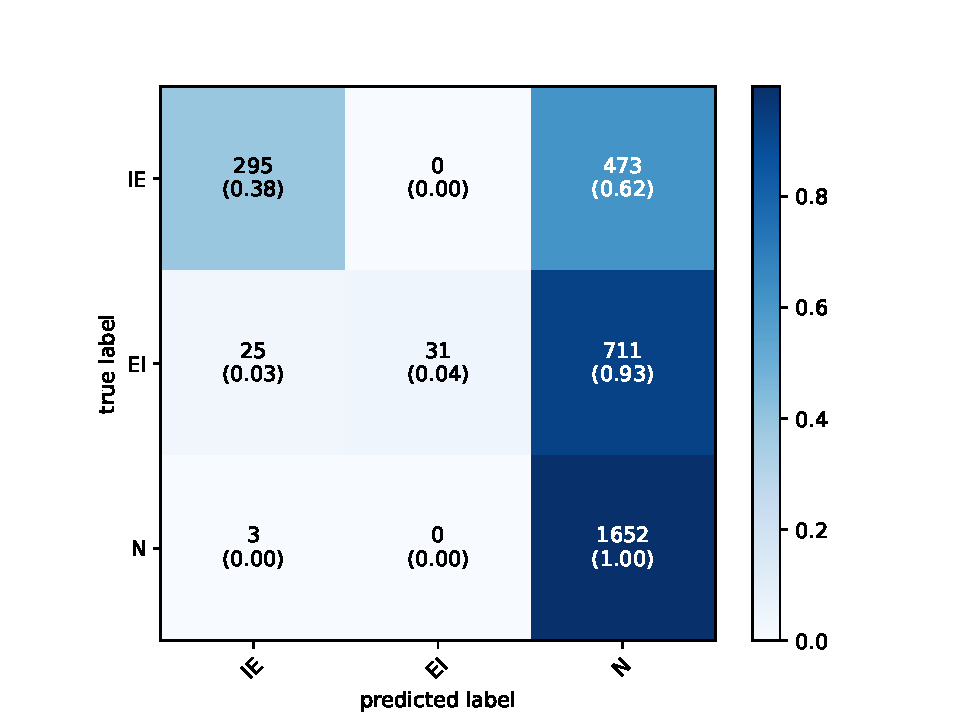
\includegraphics[width=0.6\textwidth]{figures/dna-rules-confusion-matrix}
    \end{figure}
    %
    
    \framebreak
    
    \begin{figure}
        \centering
        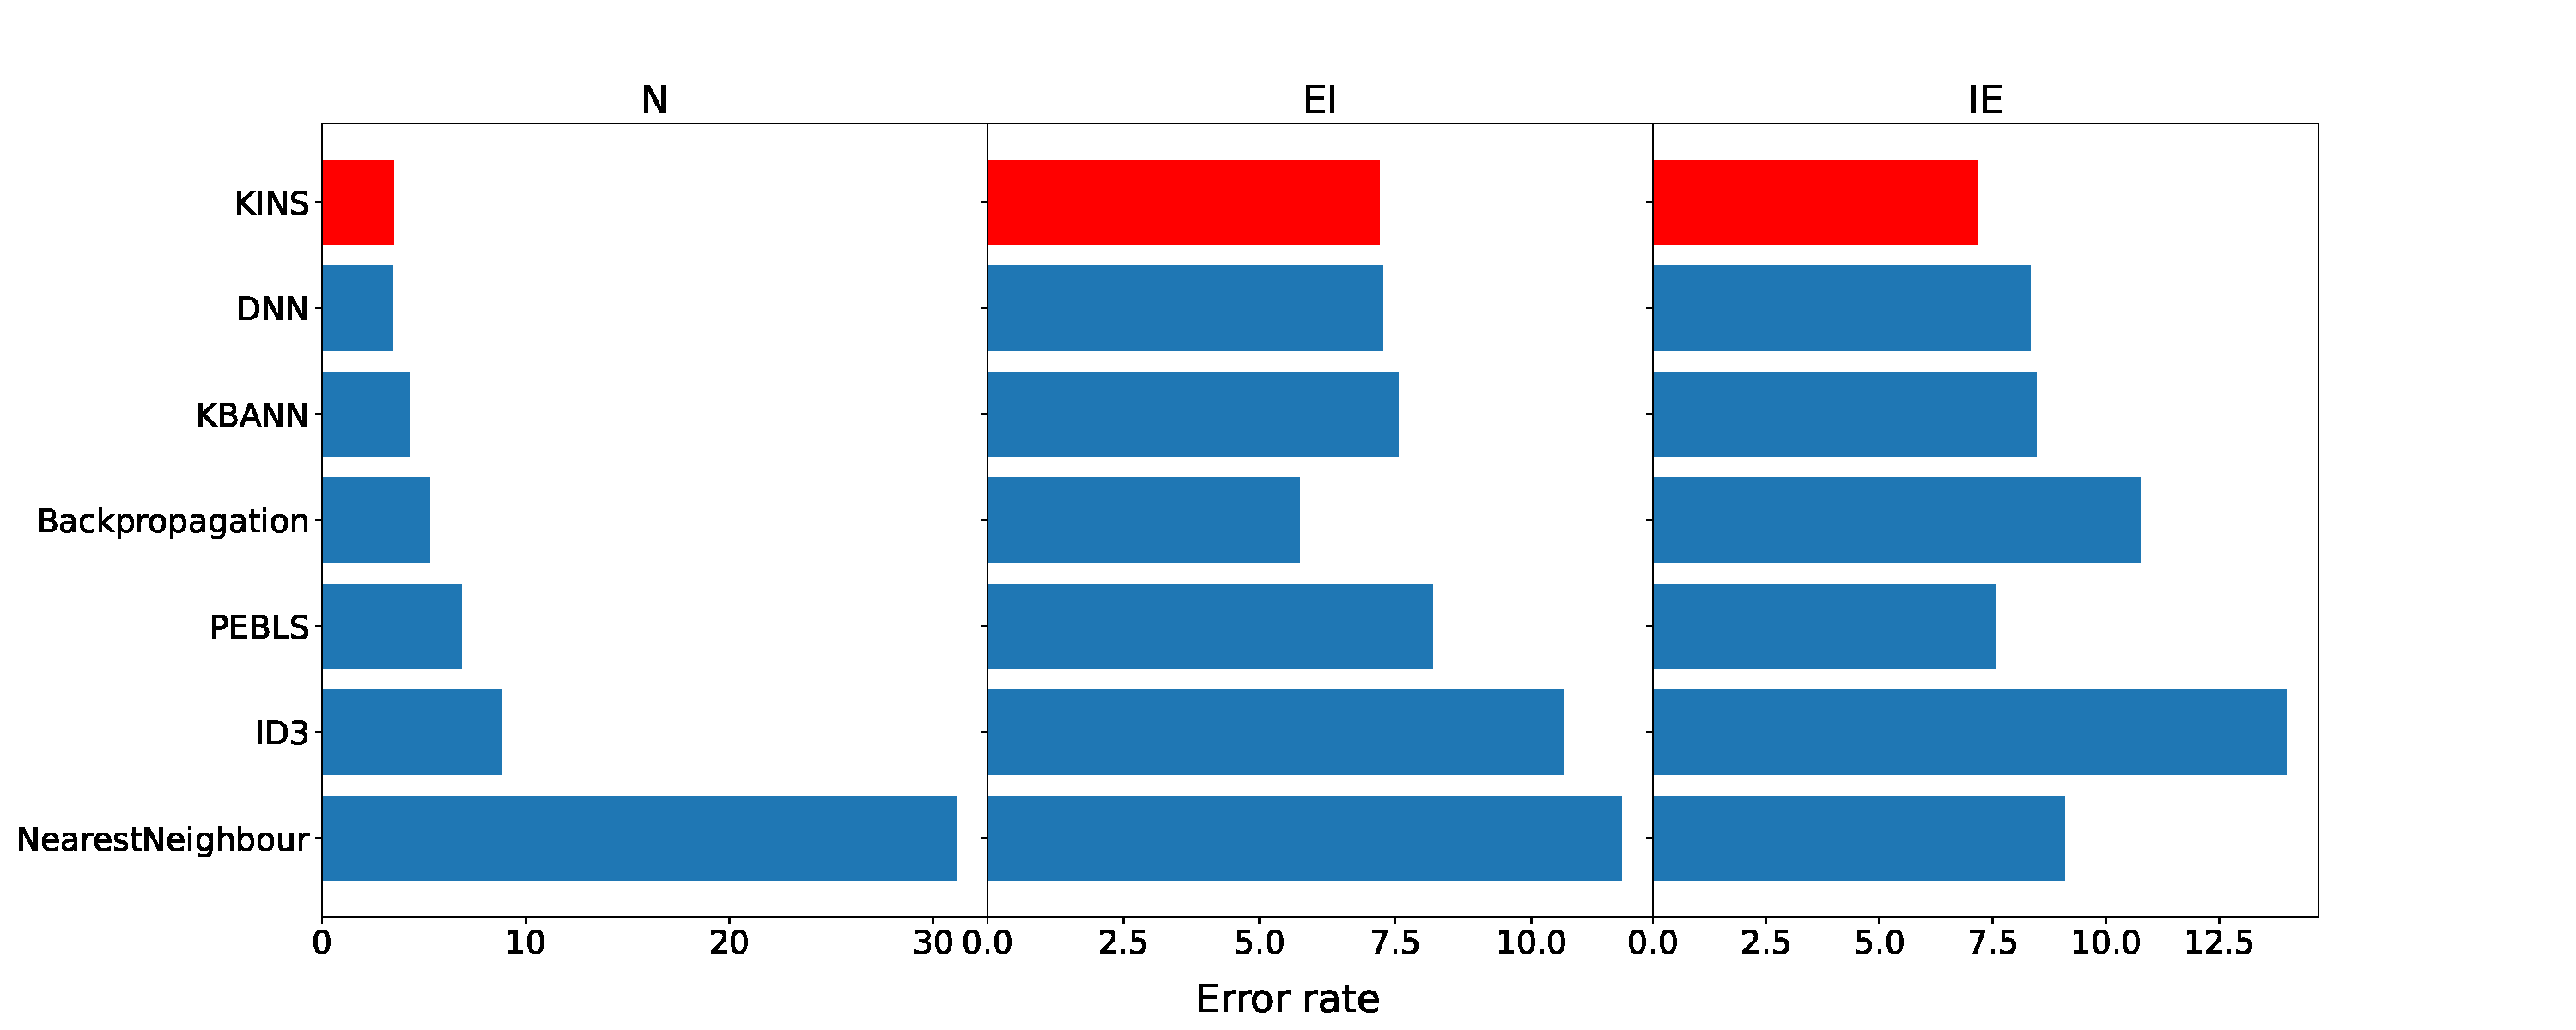
\includegraphics[width=\textwidth]{figures/kins-error-rate}
    \end{figure}
    %
    
\end{frame}
%/////////


%===============================================================================
\section{Open literature research lines}
%===============================================================================


%/////////
\begin{frame}[c]{SKE \& SKI}
    %
    \begin{figure}
        \centering
        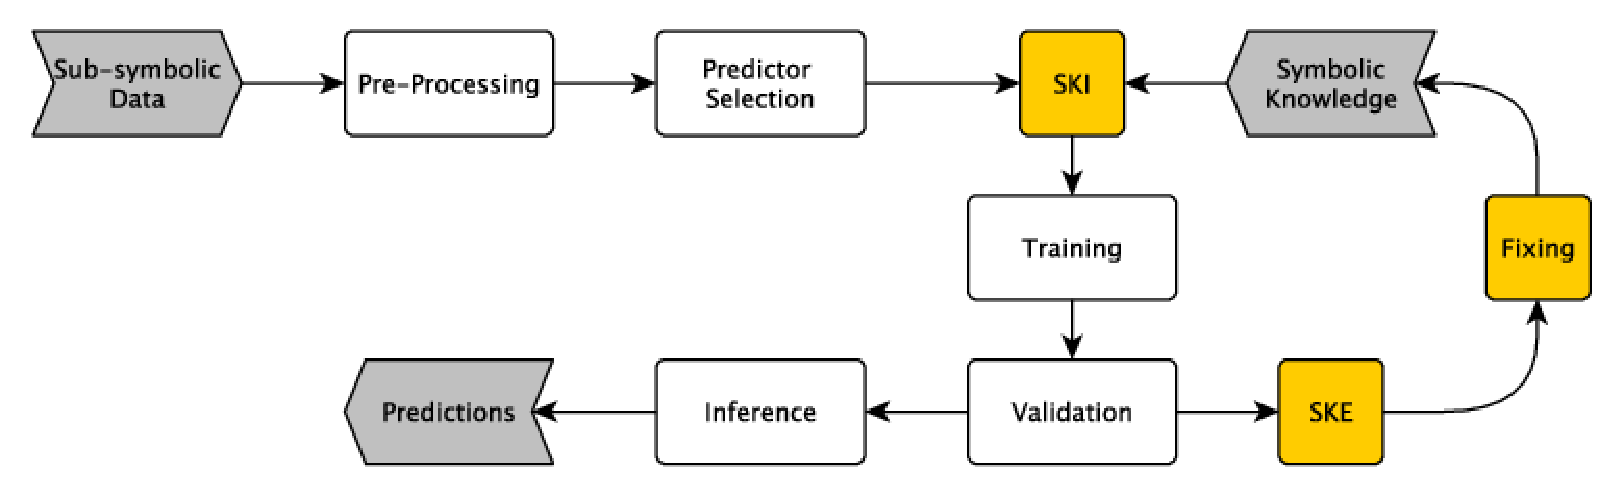
\includegraphics[width=\textwidth]{figures/ske-ski-workflow}
    \end{figure}
\end{frame}
%/////////


%/////////
\begin{frame}[c]{Multi-Agent Systems}
    %
    \begin{itemize}
        \item agent to agent explanation \ccite{explanation-aixia2020dp}\\
        %
        $\rightarrow$ SKE + SKI + explanation;
        %
        \item logic as lingua franca for communication between heterogeneous entities;
        %
        \item knowledge sharing and knowledge exploitation among agents;
        %
        \item symbolic techniques integrated with sub-symbolic ones\\
        %
        $\rightarrow$ representing and manipulating cognitive
        processes and their results.
    \end{itemize}
\end{frame}
%/////////

%===============================================================================
\section*{}
%===============================================================================

%/////////
\frame{\titlepage}
%/////////

%===============================================================================
\section*{\refname}
%===============================================================================

%%%%
\setbeamertemplate{page number in head/foot}{}
%/////////
%\begin{frame}[c,noframenumbering]{\refname}
\begin{frame}[t,allowframebreaks,noframenumbering]{\refname}
    %	\tiny
    \scriptsize
    %	\footnotesize
    \bibliographystyle{apalike-AMS}
    \bibliography{ske-ski-talk-2022}
\end{frame}
%/////////

%%%%%%%%%%%%%%%%%%%%%%%%%%%%%%%%%%%%%%%%%%%%%%%%%%%%%%%%%%%%%%%%%%%%%%%%%%%%%%%%
\end{document}
%%%%%%%%%%%%%%%%%%%%%%%%%%%%%%%%%%%%%%%%%%%%%%%%%%%%%%%%%%%%%%%%%%%%%%%%%%%%%%%%
